\section{Teoretický úvod}
  \indent\indent
  Operační zesilovač, někdy označován OZ, je zesilovač, který zesiluje rozdíl dvou napětí. Rozdílovému napětí se také někdy říká diferenciální napětí.
  
  \begin{equation}
  	U_d = U_+ - U_-
  \end{equation}
  
  \hspace*{2cm}kde:\newline    
  \hspace*{4cm}$U_{d}$ \dotfill diferenciální napětí\hspace*{4cm}\newline
  \hspace*{4cm}$U_+$ \dotfill napětí mezi neinvetujícím vstupem a pracovní zemí\hspace*{4cm}\newline
  \hspace*{4cm}$U_-$ \dotfill napětí mezi invetujícím vstupem a pracovní zemí\hspace*{4cm}\newline
  
  Operační zesilovače získali svůj název s původního záměru jejich vytvoření. Byly stvořeny za účelem provádění aritmetických operací nad analogovými signály. První OZ s elektronkamy skunstruoval roku 1938 G.~A.~Philbrick. Pozdeji byli elektronky nahrazaovány tranzistory. Zdokonalení výrobních postupů nám umožnilo začít vyrábět operační zesilovače integrované do jednoho čipu.
  
  \subsection{Ideální operační zesilovač}
  	\indent\indent	
  	Zesílení ideální operační zesilovač je nekonečně velké. Má nekonečně velký vstupní odpor a nulový výstupní odpor. Jeho odezva je okamžitá a jeho výstup je závislí pouze na diferenciálním napětí. Dokáže zpracovávat signáli které mají vyšší napětí než je napájecí napětí tohoto OZ. Výstupní napětí Ideálního OZ je dáno vstahem:  	
  	
		\begin{equation}
			U_{OUT} = A_u\cdot U_d
		\end{equation}
		
		\hspace*{2cm}kde:\newline    
    \hspace*{4cm}$U_{OUT}$ \dotfill výstupní napětí\hspace*{4cm}\newline
    \hspace*{4cm}$U_d$ \dotfill diferenciální napětí\hspace*{4cm}\newline
    \hspace*{4cm}$A_u$ \dotfill napěťové zesílení OZ\hspace*{4cm}\newline
	  
  \subsection{Neinvertující zapojení OZ}
    \indent\indent
    Toto zapojení neposouvá fázi výstuního napětí. Výstupní napětí je dáno poměrem rezistorů $R_1$ a $R_2$. Odvození vztahů pro OZ zapojený v neinvertujícím zapojení za předpokladu, že OZ je ideální:
    
    \begin{eqnarray}
      U_d &=& 0 \nonumber\\
      U_d &=& U_+ - U_- \nonumber\\      
      U_+ &=& U_- = U_{IN} \nonumber\\
      I_1 &=& I_2 \nonumber\\
      U_- &=& \dfrac{R_1}{R_1+R_2}\cdot U_{OUT} \nonumber\\
      U_{OUT} &=& A_N \cdot U_+ \nonumber\\      
      A_N &=& \dfrac{U_{OUT}}{U_{IN}} = \dfrac{U_{OUT}}{\dfrac{R_1}{R_1+R_2}\cdot U_{OUT}} = \dfrac{1}{\dfrac{R_1}{R_1+R_2}} = \dfrac{R_1+R_2}{R_1}\nonumber\\
      A_N &=& 1+\dfrac{R_2}{R_1}
    \end{eqnarray}
    
    \clearpage
    \hspace*{2cm}kde:\newline    
    \hspace*{4cm}$U_{OUT}$ \dotfill výstupní napětí\hspace*{4cm}\newline
    \hspace*{4cm}$U_{IN}$ \dotfill vstupní napětí\hspace*{4cm}\newline
    \hspace*{4cm}$U_d$ \dotfill diferenciální napětí\hspace*{4cm}\newline    
    \hspace*{4cm}$U_+$ \dotfill napětí mezi neinvetujícím vstupem a pracovní zemí\hspace*{4cm}\newline
  	\hspace*{4cm}$U_-$ \dotfill napětí mezi invetujícím vstupem a pracovní zemí\hspace*{4cm}\newline
  	\hspace*{4cm}$A_N$ \dotfill napěťové zesílení danné poměrem rezistorů $R_1$ a $R_2$\hspace*{4cm}\newline
  	\hspace*{4cm}$R_1$ \dotfill rezistor\hspace*{4cm}\newline
  	\hspace*{4cm}$R_2$ \dotfill rezistor\hspace*{4cm}\newline
  	\hspace*{4cm}$I_1$ \dotfill proud\hspace*{4cm}\newline
  	\hspace*{4cm}$I_2$ \dotfill proud\hspace*{4cm}\newline
  	
    
    \begin{figure}[H]
		  \centering
		  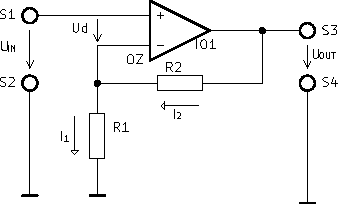
\includegraphics[width=12cm]{../img/nei.pdf}
		  \caption{Neinvertující zapojení OZ}
		  \label{sch:nei}
  	\end{figure}
  
  
    
  \subsection{Invertující zapojení OZ}
    \indent\indent
    Toto zapojení posouvá fázi o $\pi$. Odvození vztahů pro OZ zapojený v invertujícím zapojení za předpokladu, že OZ je ideální:
    
    \begin{eqnarray}
      U_d &=& 0 \nonumber\\
      U_d &=& U_+ - U_- \nonumber\\      
      U_+ &=& U_- = U_{IN} \nonumber\\
      I_1 &=& -I_2 \nonumber\\
      U_{IN} &=& I_1 \cdot R_1 \nonumber\\
      U_{OUT} &=& -I_1 \cdot R_2 \nonumber\\
      A_N &=& \dfrac{U_{OUT}}{U_{IN}} = -\dfrac{I_1 \cdot R_2}{I_1 \cdot R_1} \nonumber\\
      A_N &=& -\dfrac{R_2}{R_1}
    \end{eqnarray} 
    
    \clearpage
    \hspace*{2cm}kde:\newline    
    \hspace*{4cm}$U_{OUT}$ \dotfill výstupní napětí\hspace*{4cm}\newline
    \hspace*{4cm}$U_{IN}$ \dotfill vstupní napětí\hspace*{4cm}\newline
    \hspace*{4cm}$U_d$ \dotfill diferenciální napětí\hspace*{4cm}\newline    
    \hspace*{4cm}$U_+$ \dotfill napětí mezi neinvetujícím vstupem a pracovní zemí\hspace*{4cm}\newline
  	\hspace*{4cm}$U_-$ \dotfill napětí mezi invetujícím vstupem a pracovní zemí\hspace*{4cm}\newline
  	\hspace*{4cm}$A_N$ \dotfill napěťové zesílení danné poměrem rezistorů $R_1$ a $R_2$\hspace*{4cm}\newline
  	\hspace*{4cm}$R_1$ \dotfill rezistor\hspace*{4cm}\newline
  	\hspace*{4cm}$R_2$ \dotfill rezistor\hspace*{4cm}\newline
  	\hspace*{4cm}$I_1$ \dotfill proud\hspace*{4cm}\newline
  	\hspace*{4cm}$I_2$ \dotfill proud\hspace*{4cm}\newline
    
    \begin{figure}[H]
		  \centering
		  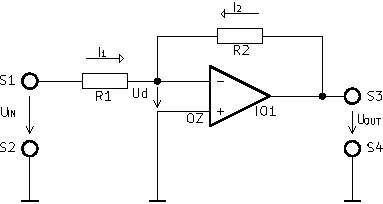
\includegraphics[width=14cm]{../img/inv.pdf}
		  \caption{Invertující zapojení OZ}
		  \label{sch:inv}
  	\end{figure}
    
    
  \subsection{MAA741}
  	MAA741 je obvod, ve kterého je integrován operační zesilovač. Tento obvod se vyrábí v pouzdrech TO-99, CDIP-8, PDIP-8 a CLGA. Jeho klíčové parametry jsou shrnuty v tabulce 1.
  	
  	\begin{table}[H]
		  \begin{center}
		    \begin{tabular}[H]{!{\vrule width 1pt}c|c|c!{\vrule width 1pt}}
		      \specialrule{1pt}{0pt}{0pt} 
		      \textbf{veličina} & \textbf{označení veličiny} & \textbf{hodnota} \\\specialrule{1pt}{0pt}{0pt} 
		      Napájecí napětí& $U_{CC}$ & $\pm3~V~ ... \pm22~V$ \\\hline
		      Napájecí proud & $I_{CC}$ & $1,3~mA~ ... ~2,8~mA$ \\\hline
		      Diferenciální napětí & $U_d$ & $\pm30~V$ \\\hline
		      Vstupní napětí & $U_I$ & $\pm15~V$ \\\hline
		      Ztrátový výkon & $P_{tot}$ & $500~mW$ \\\hline		      
		      Napěťové zesílení OZ & $A_u$ & $50 000 ~ ... ~150 000$ \\\hline
		      Rozsah pracovních teplot & $\vartheta_a$ & $-55~^\circ C~...~+125~^\circ C$ \\\specialrule{1pt}{0pt}{0pt} 
		      
		    \end{tabular}
		    
		    \caption{Hlavní parametry MAA741}
		    \label{tab:s1}      
		  \end{center}
		\end{table}
		
		\begin{figure}[H]
		  \centering
		  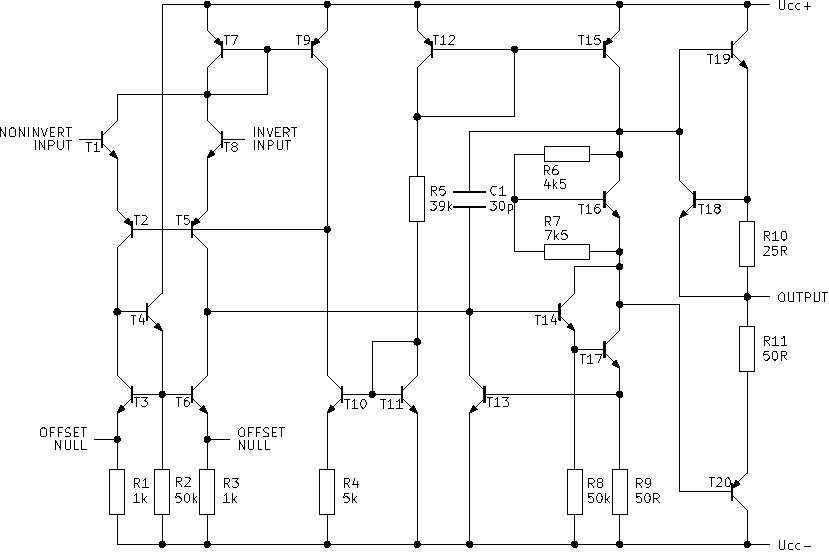
\includegraphics[width=15cm]{../img/MAA741.pdf}
		  \caption{Vnitřní zapojení MAA741}
		  \label{sch:vz}
  	\end{figure}
   
  
